\documentclass{article}

\usepackage[margin=1in]{geometry}
\usepackage{enumerate}
\usepackage{enumitem}
\usepackage{graphicx}
\usepackage{subfig}
\usepackage{amsmath}
\usepackage{multirow}
\usepackage{hyperref}
\hypersetup{
    colorlinks=true,
    linkcolor=blue}


\begin{document}
\begin{titlepage}
	\clearpage\thispagestyle{empty}
	\centering
	\vspace{1cm}
		
	\rule{\linewidth}{1mm} \\[0.5cm]
	{ \Large \bfseries ISyE 6740 - Summer 2021\\[0.2cm]
	    Project Report \\[0.5cm]
		Firm Strategy and Financial Performance with Natural Language Processing\\[0.5cm]
		Erik Magnusson 903661584\\[0.01cm]
		Jos Vilier 903638166\\[0.01cm]
		Vera Thut 903560685\\[0.01cm]}
	\rule{\linewidth}{1mm} \\[1cm]
\end{titlepage}

{
  \hypersetup{linkcolor=black}
  \tableofcontents
}
\newpage

\section{Problem statement}
Firm strategy is big business. There are countless MBA students, financial analysts, and consultants searching for the optimal business strategy. In the following analysis, we employ machine learning techniques to identify firm strategies and quantify their effects on financial performance. 

Firm strategy is a result of topics that are top of mind for the firm. There are many ways in which firms try to achieve competitive advantage depending on what they believe are the most important strategic factors. For example:
\begin{itemize}
    \item Firms may choose to "go green" if they are concerned about climate change
    \item Firms can focus on differentiation if they believe consumer behavior is changing
    \item Firms can focus on cutting costs if they deem their products interchangeable with their competitors
\end{itemize}
In this project, we measure how a firm's performance is affected by its strategic choices. The textbook answer would be yes: a firm that makes good strategic choices will be able to generate more revenues and/or reduce costs, leading to additional profits. These additional profits would be reflected in a higher stock price. 

\clearpage
\section{Data sources}

The two main data inputs for this analysis are firm strategy and financial performance, collected as text files and time series, respectively. 

The analysis is restricted to firms in the consumer packaged goods (CPG) food industry. Because of the common consumer-facing nature of this sector, many people are familiar with these companies and can understand their business structures and strategies with relative ease. It is also a large sector with many publicly traded companies, providing a large selection of available annual reports for analysis. The CPG companies used in this analysis are restricted to firms in the S\&P 500 Index to ensure that the components of the holding period return are freely available.

\subsection{Firm strategy}
Firm strategy is particularly hard to capture, as it is not a quantitative variable that firms are required to publish. However, all publicly traded companies in the United States are required to file their annual reports with the US Securities and Exchange Commission (SEC). The SEC stores this information in their database \href{https://www.sec.gov/edgar.shtml}{EDGAR}.

 The reports follow a standard template. Most information is accounting related, e.g., a balance sheet and profit and loss statement over the calendar year. Each report is largely backward-looking, focusing on the company's past performance. However, every report contains a Risk Factors section that is always forward-looking. This is where a firm identifies and manages risks that may threaten their business in the short and long term. It generally includes subjects such as increased regulation, climate change, changing consumer preferences and potential litigation. It contains valuable information about the topics that are top of mind at the firm and may shape firm strategy. By extracting the text in these risk sections, we generated a data set for identifying patterns regarding firm strategy. 

The qualitative parts of annual reports (such as the risk factor section) are generally written in November and December of the calendar year. For example, the 2018 annual reports (containing profits and losses for the year 2018) tends to be published in March or April 2019, but the risk factor section was written in November 2018 and focuses on potential risks in 2019 and beyond. For this reason we are going to link the annual report over 2018 to the financial performance over 2019. We also choose to exclude the year 2020 from the data set, because the pandemic would lead to many outliers. Furthermore, to reduce the influence of autocorrelation we do not include consecutive years. We chose to use one in every three years for this reason. Going back further in time may lead to data availability issues, hence we restrict ourselves to 2012 and further. Table \ref{tab:data_cohorts} contains what years are selected.

We used annual reports from 14 companies and have total of 39 observations in our data set. The annual reports were uploaded from \href{https://www.annualreports.com/}{AnnualReports} in PDF format. As formatting in the annual reports varies, the Risk Factors data was manually extracted from each of the report and converted to individual .txt files. 

\begin{table}[h]
    \centering
    \begin{tabular}{c|c|c}
        \textbf{Cohort} & \textbf{Annual report} & \textbf{Return} \\
        \hline
         1 & 2012 & 2013 \\
         2 & 2015 & 2016 \\
         3 & 2018 & 2019
    \end{tabular}
    \caption{Years in the data set}
    \label{tab:data_cohorts}
\end{table}

\subsection{Financial performance}
Unlike firm strategy, financial performance is relatively easy to quantify. Financial performance is calculated using the difference between the annual return of a given public company, adjusted for dividends and events like stock splits, and the overall annual return of the S\&P 500 Index. This calculation generates the company's excess returns for a given year and is used as the benchmark for financial performance.

Each company's financial performance is captured using the \href{https://www.alphavantage.co/}{Alpha Vantage API}, which returns JSON-formatted time series stock data. This contains historical daily close prices for public companies, as well as any relevant stock split/dividend event data. By executing an API call for each of the consumer packaged goods companies of interest, we obtain 20+ years of historical financial performance data. 

\begin{figure}[ht]
    \centering
    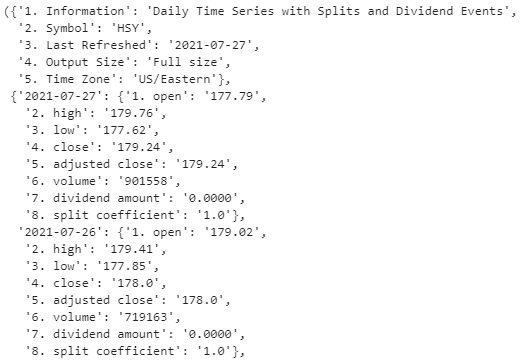
\includegraphics[width = 0.6\linewidth]{AlphaVantage_HSY}
    \caption{Alpha Vantage API output: Hershey (HSY) example}
    \label{fig:AlphaVantage_HSY}
\end{figure}

Historical S\&P 500 Index returns are available through \href{https://www.berkshirehathaway.com/letters/2019ltr.pdf}{Berkshire Hathaway} and are assumed to represent an estimate of overall market return for a given year. Subtracting these market returns from the corresponding adjusted annual returns for each CPG company yields the financial performance benchmark for this analysis. Because annual reports from the years 2012, 2015, and 2018 are being considered, excess returns for the years 2013, 2016, and 2019 are calculated. 

\clearpage
\section{Methodology}
The methodology consists of three steps. There are two options for the third step, which will both be explored to ensure robustness of the results. The steps are explained in more detail below.

\subsection{Natural language processing}
In this step we convert the risk factor section in the annual reports to a vector that captures the topics that are top of mind at the firm. We do this by applying a bag of words model, which simply consists of counting how often each word is used. There will likely be a step in this process where we specify what words should be considered (i.e. what are the features). For example, the word "is" will likely be used very often, but it does not convey information regarding firm strategy. These words will be removed from the feature vector. This step is performed manually and can be rather subjective. The selected and removed words are available in "/data/bag of words/bow\_unfiltered\_tagged.xlsx". 422 out of 5,651 unique words are selected. Note that so called stop words are filtered for as well. 

It is important to realize that the total number of words can be very different from one annual report to the next, hence we correct for this by standardizing with the overall word count per annual report.

The result of this step is a matrix that contains the relative word count for each observation (row) for every considered word (column). The rows sum up to 1. An example is given in table \ref{tab:bow}. The size of the matrix is 42 (firms) by 422 (unique words related to strategy). The matrix is rather sparse.

\begin{table}[h]
    \centering
    \begin{tabular}{c|c|c|c|c|c|c}
        \textbf{Firm \& Year} & \textbf{Accountants} & \textbf{Accounting} & \textbf{Acquire} & \textbf{...} & \textbf{Workforce} \\
        \hline
        ADM\_2012 & 0 & 0.005 & 0 & ... & 0.005 \\
        ADM\_2015 & 0 & 0.004 & 0 & ... & 0.004 \\
        ADM\_2018 & 0 & 0.003 & 0 & ... & 0.003 \\
        ... & ... & ... & ... & ... & ... \\
        TR\_2018 & 0 & 0.006 & 0 & ... & 0 \\
    \end{tabular}
    \caption{Bag of words results}
    \label{tab:bow}
\end{table}

Over all of the annual reports in the data set, the 20 most common words, measured by the sum of their relative frequencies, are shown in Figure \ref{fig:BoW_Bar_Chart}. Many of the most frequently used words could be considered generic commercial terminology, such as "business", "financial", and  "customers". However, the manner in which an organization stresses these different components could provide insight into broader strategic intent.

\begin{figure}[ht]
    \centering
    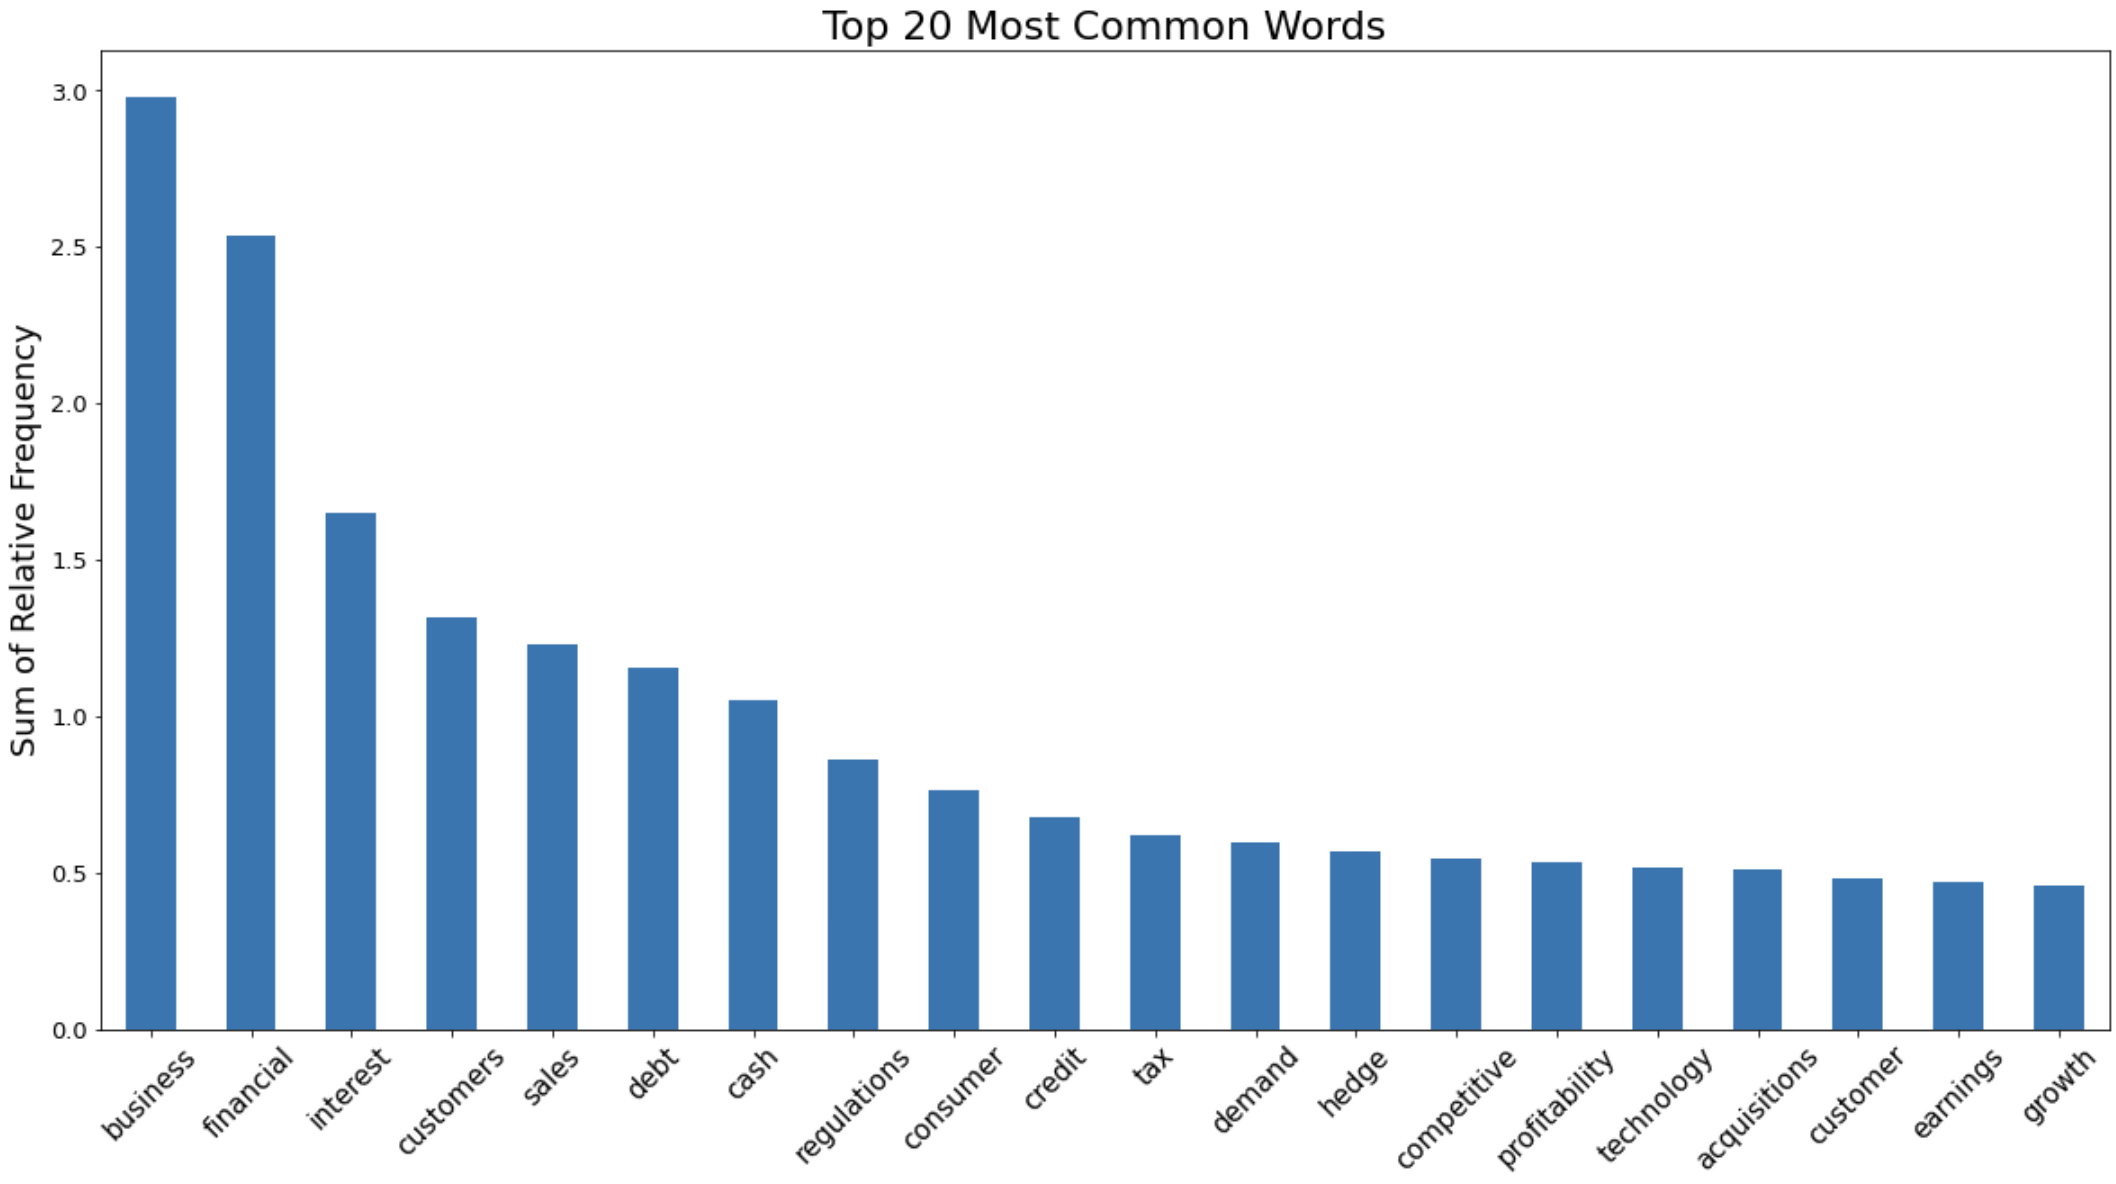
\includegraphics[width = 0.8\linewidth]{BoW_Bar_Chart.png}
    \caption{Most common words, by relative frequency, in annual report risk factor sections}
    \label{fig:BoW_Bar_Chart}
\end{figure}

For example, Figure \ref{fig:wordcloud} shows two word clouds from example annual reports in the data set. Common terminology like "business", "financial", "growth", and "data" are mentioned frequently in both the HSY and ADM 2018 annual reports. However, in addition to the high usage of those shared terms, each company differentiates its strategic focus by repeatedly using more specific terminology. For example, HSY has higher relative word frequencies for "customers", "sales", "energy", and "technology", while ADM has higher relative word frequencies for "regulations", "compliance", "credit", and "reputation".

\begin{figure}[ht]
    \centering
    \subfloat[\centering HSY 2018 Annual Report]{{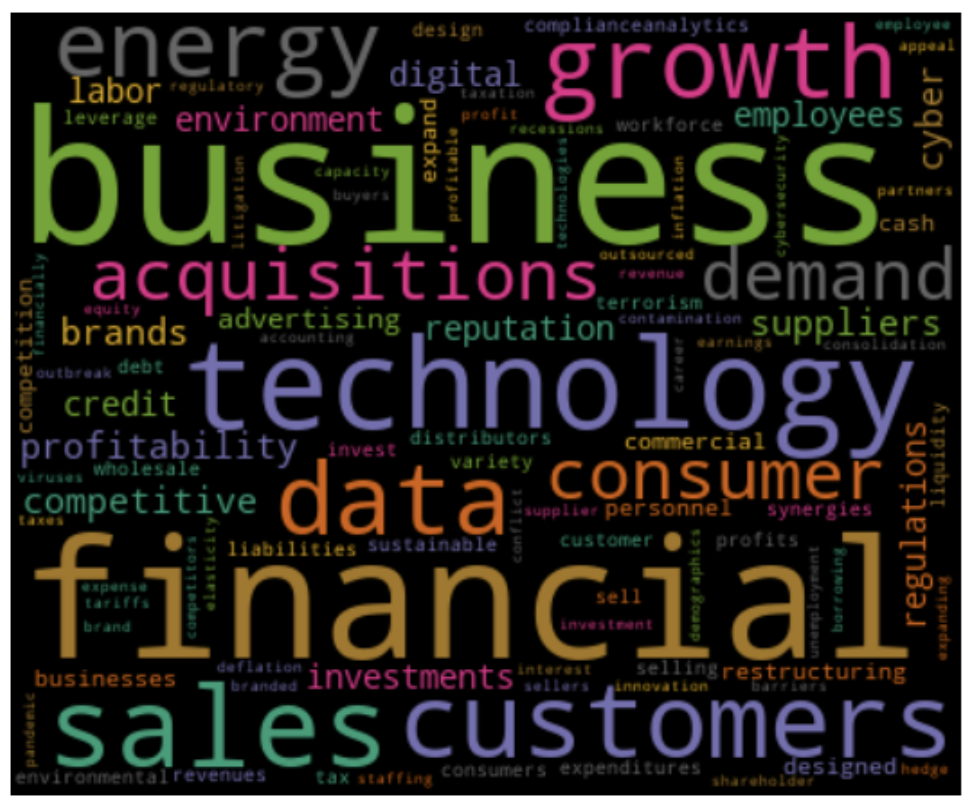
\includegraphics[width=5cm]{HSY_2018_wordcloud} }}%
    \qquad
    \subfloat[\centering ADM 2018 Annual Report]{{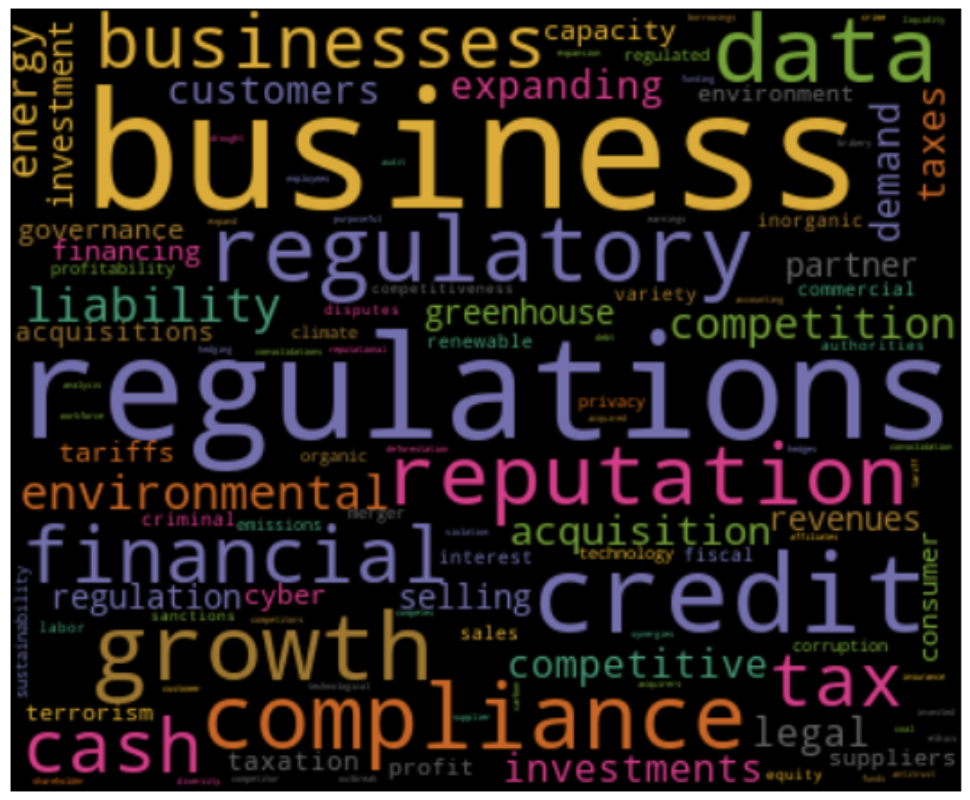
\includegraphics[width=5cm]{ADM_2018_wordcloud} }}%
    \caption{Example word frequencies for Risk Factors sections}%
    \label{fig:wordcloud}%
\end{figure}

\subsection{Dimensionality reduction}
The number of word frequency features generated by the bag of words analysis (n = 422) is much greater than the number of observations (m = 42) in the data set. To avoid having more predictors than observations, which can lead to issues like overfitting, principal component analysis (PCA) is used to reduce dimensionality. This is accomplished by projecting the original data set onto the first few principal components, belonging to an orthonormal basis of the original feature space, in an effort to reduce the number of features while maximizing the amount of data variation retained.

PCA allows us to recognize which word combinations account for the most variation between observations and provides insights into the strategies being discussed in each annual report. Figure \ref{fig:PCA_cum_var_plot} displays the proportion of overall variance from the original data set that is explained by each subsequent principal component. Given the dimensions of the data set, the most effective modeling will come from minimizing the number of principle components used while maximizing their cumulative explained variance.

\begin{figure}[ht]
    \centering
    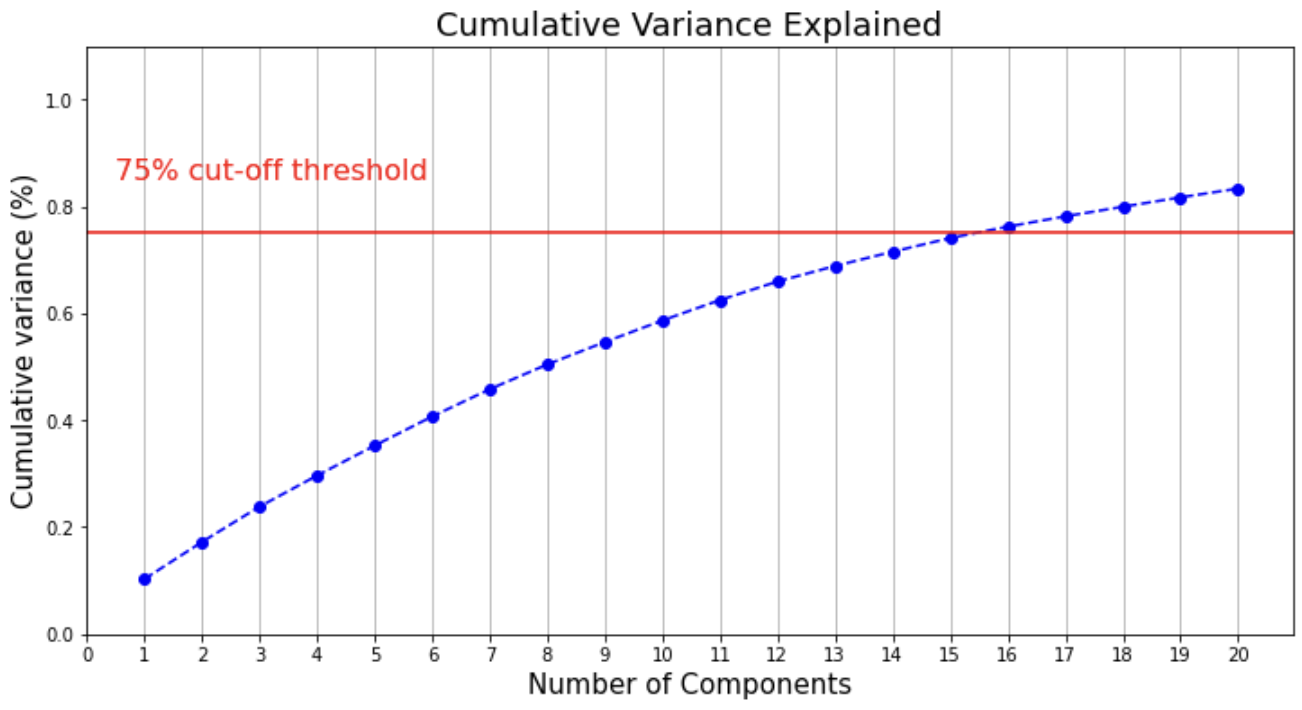
\includegraphics[width = 0.7\linewidth]{PCA_cum_var_plot}
    \caption{Cumulative variance explained by the first 20 principle components}
    \label{fig:PCA_cum_var_plot}
\end{figure}

While it would be ideal to select a number of principle components that explains a cumulative variance percentage closer to the arbitrary 75\% threshold shown in Figure \ref{fig:PCA_cum_var_plot}, it would be counterproductive given the small annual report sample size. Also, as seen in Figure \ref{fig:PCA_explainedvariance}, there is no sudden drop off in explained variance between the different components, creating a situation in which there is no natural number of components that should be considered. This leads to a bias-variance trade-off which depends on the number of principle components included in the analysis. Including more principle components allows more of the original variance in the data to be incorporated in the modeling process. However, introducing too many features relative to the number of observations can lead to increased variance when generalizing to new data.

\begin{figure}[ht]
    \centering
    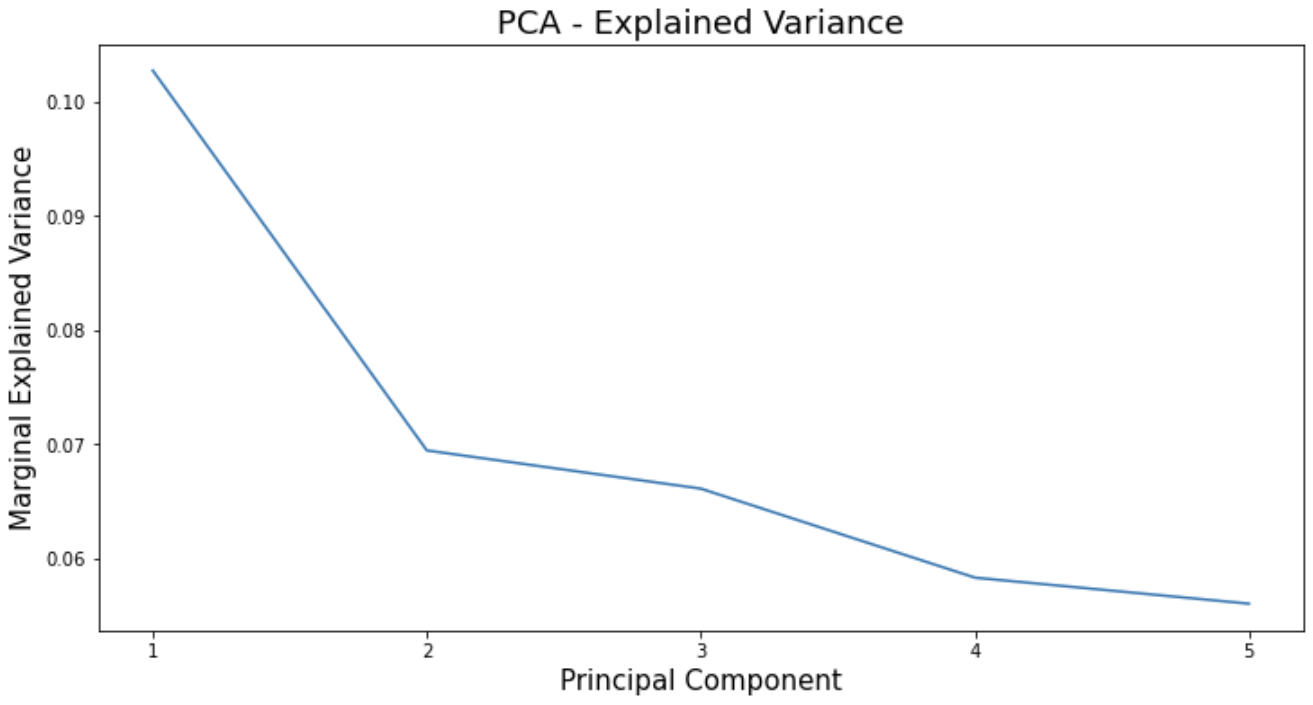
\includegraphics[width = 0.7\linewidth]{PCA_explainedvariance}
    \caption{Marginal variance explained by the first 5 principal components }
    \label{fig:PCA_explainedvariance}
\end{figure}

We decided to go with five components to be able to capture a wide range of strategies. Table \ref{tab:PCA} contains the five words associated with the largest (positive) and smallest (negative) values for each component. 

\begin{table}[ht]
    \centering
    \begin{tabular}{c|c|c|c|c|c}
        & \textbf{Component 1} & \textbf{Component 2}& \textbf{Component 3}& \textbf{Component 4}& \textbf{Component 5} \\
        \hline
        \multirow{5}{*}{Positive} & Noncompliance & Acquired & Reputation & Analysts & Expenditures \\
        &Pollution & Brand & Regulatory & Affordably & Acquisitions\\
        &Afford & Brands & Selling & Analyst & Profitability \\
        &Commercialization & Patent & Cyber & Appealing & Pandemic \\
        &Compliant & Consumers & Invested & Budgets & Demographic \\
        \hline
        \multirow{5}{*}{Negative} & Energy & Energy & Debt & Sellers & Interest \\
        & Environment & Demand & Cash & Distributors & Hedged \\
        & Competitive & Outbreak & Acquire & Buyers & Hedge \\
        & Pandemic & Hedge & Interest & Employee & Accounting \\
        & Cyber & Terrorism & Earnings & Innovation & Bribery \\
        \hline
    \end{tabular}
    \caption{Principal component analysis results}
    \label{tab:PCA}
\end{table}

These words allow for interpretation of the principal components. For example, the words "energy", "environment", "competitive", "pandemic" and "cyber" are commonly used in reports that have a low value for the first component. This indicates that the firm is concerned about catastrophes because all words except "competitive" are associated with catastrophes. Positive values for the first component indicate that they are concerned about compliance issues e.g. with food and drug authority rulings ("noncompliance", "compliant") and commercial aspects ("afford", "commercialization"). The components have been analyzed and translated into strategies in table \ref{tab:PCA_meaning}. The strategy indicates what the firm focuses on. 

This step is rather subjective. There are a number of ways in which this analysis can be improved, e.g. by correcting for synonyms, by collecting more data or by considering more than the top five words to decide on the strategy. All these approaches require substantial time investments however.

\begin{table}[h]
    \centering
    \begin{tabular}{c|c|c}
        \textbf{Component} & \textbf{Positive} & \textbf{Negative} \\
        \hline
         1 & Compliance issues and commercial aspects & Catastrophes \\
         2 & Marketing and consumer needs & Catastrophes \\
         3 & Compliance issues & Financial aspects \\
         4 & Consumer needs & Competitive environment \\
         5 & Mergers and acquisitions & Financial aspects 
    \end{tabular}
    \caption{Component interpretation}
    \label{tab:PCA_meaning}
\end{table}


\subsection{Classification and clustering}
In this section we are going to test in two ways whether there is any link between firm strategy and financial performance. The following two approaches both start after the PCA step, hence the project branches off in two models. We apply clustering and classification to analyze the results.

\subsubsection{Clustering}
Approach number one starts with clustering of the observations. Next we are going to compute the average outperformance of the S\&P 500 for each cluster and compare these. Large differences between this outperformance are indicators that strategy indeed plays a role to explain financial performance. The clustering is done by the well known k-means model based on Euclidean distances. The PCA data is standardized before applying the model.

The sum of squared distances (also known as residuals) are plotted as a function of the number of cluster centers in figure \ref{fig:kmeans}.  

\begin{figure}[!ht]
    \centering
    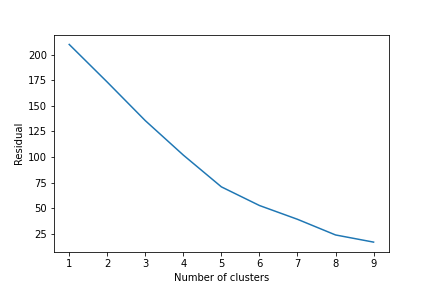
\includegraphics[width = 0.6\linewidth]{kmeans}
    \caption{Residuals for the k-means model}
    \label{fig:kmeans}
\end{figure}

The graph does not show a clear elbow point. The most likely candidates are k = 5 and k = 8, however those are rather high cluster numbers with only 42 observations. We decided to go with k = 3, which leads to the clustering in table \ref{tab:kmeans1} and cluster centers in table \ref{tab:kmeans2}. Note that we did not have three years of history for ANFI and NOMD.

\begin{table}[htb]
    \centering
    \begin{tabular}{c|c|c}
        \textbf{Cluster 0} & \textbf{Cluster 1} & \textbf{Cluster 2}\\
        \hline
        ANFI\_2015 & ADM\_2012 & BGS\_2012 \\
        ANFI\_2018 & ADM\_2015 & BGS\_2015 \\
        & ADM\_2018 & BGS\_2018 \\
        & HSY\_2012 & CAG\_2012 \\
        & HSY\_2015 & CAG\_2015 \\
        & HSY\_2018 & CAG\_2018 \\
        & INGR\_2012 & CPB\_2012 \\
        & INGR\_2015 & CPB\_2015 \\
        & INGR\_2018 & CPB\_2018 \\
        & SJM\_2012 & K\_2012 \\
        & SJM\_2015 & K\_2015 \\
        & SJM\_2018 & K\_2018 \\
        & TR\_2012 & MKC\_2012 \\
        & TR\_2015 & MKC\_2015 \\
        & TR\_2018 & MKC\_2018 \\
        & GIS\_2012 & GIS\_2018 \\
        & GIS\_2015 & NOMD\_2018 \\
        & & POST\_2012 \\
        & & POST\_2015 \\
        & & POST\_2018 \\
        & & THS\_2012 \\
        & & THS\_2015 \\
        & & THS\_2018 
    \end{tabular}
    \caption{Clusters for k = 3}
    \label{tab:kmeans1}
\end{table}

The clustering shows that ANFI is so different from the other reports that it gets it own cluster. In addition, the clustering seems to capture that there is autocorrelation between the different years, as almost all firms remain in their cluster (GIS is the only exception). Cluster 1 and 2 are both reasonably populated compared to cluster 0. 

\begin{table}[htb]
    \centering
    \begin{tabular}{c|c|c|c|c|c}
        \textbf{Cluster} & \textbf{Component 1} & \textbf{Component 2}& \textbf{Component 3}& \textbf{Component 4}& \textbf{Component 5} \\
        \hline
        0 & 3.97 & -1.19 & 0.39 & -1.07 & 0.02 \\
        1 & -0.47 & -0.97 & 0.18 & 0.25 & -0.05 \\
        2 & 0.00 & 0.82 & -0.16 & -0.09 & 0.04 
    \end{tabular}
    \caption{Cluster centers for k = 3}
    \label{tab:kmeans2}
\end{table}

The cluster centers for cluster 1 and 2 are not that different. It is mainly component 2 where the centers are quite far apart. Resorting back to the strategies in table \ref{tab:PCA_meaning} shows that cluster 1 mainly focuses on catastrophes (as the value of component 2 is negative), while cluster two focuses on marketing and consumer needs (as the value of component 2 is positive). Cluster 0 stands out in the first component. The results for cluster 0 are not that interesting however, as it seems to capture an outlier only.

The average outperformance for each cluster are -40.7\%, -0.6\% and -3.7\%. This shows that the CGP food industry performed worse than the S\&P500 in general, but cluster 1 had a stronger performance compared to cluster 2. This seems to indicate that it is better to focus on catastrophes than marketing and consumer needs. However, the performance may also be (subtly) influenced by the other components (or strategies), hence we will take a closer look at all components in the following section on classification models.

\clearpage

\subsubsection{Classification}
For our analysis, we used a number of supervised learning algorithms to understand whether features can predict outperformance (return higher than S\&P 500) or underperformance (return lower than S\&P 500) of a particular company.

Supervised Learning models used: 
\begin{itemize}
    \item \textbf{Naive Bayes}.\\
    Strengths: This model can deal with many features. It is simple and fast.\\ 
    Limitations: classifier assumes that all attributes are mutually independent. 
    \item\textbf{KNN}.\\
    Strengths: This algorithm is easy to implement and rather versatile.\\
    Limitations: it can get slow, as the number of features increases. 
    \item \textbf{Logistic Regression}.\\ 
    Strengths: This classifier is easy to implement, it is also less prone to over-fitting. \\
    Limitations: it is hard to understand complex relationships using this algorithm. 
    \item \textbf{Linear SVM}\\
    Strengths: Effective for high-dimensional data sets. Memory efficient.\\
    Limitations: Does not perform well for data set with a lot of noise. Can under perform if number of features exceeds number of training data samples.
\end{itemize}

Out or under performing S\&P 500 was defined as a Target Variable. The data was split 70/30 for train/test. The classifiers were run using the calculated principle components as features. We experimented utilizing varying numbers of principle components: 2, 3 and 5. Below are the accuracy scores for each classifier with each different set of principle components: 

\begin{table}[htb]
    \centering
    \begin{tabular}{c|c|c|c|c|c}
        \textbf{Data} & \textbf{Naive Bayes} & \textbf{KNN}& \textbf{Logistic Regression}& \textbf{Linear SVM}\\
        \hline
        5 principle components & 0.55 & 0.4 & 0.4 & 0.4  \\
        3 principle components & 0.6 & 0.5 & 0.5 & 0.45  \\
        2 principle components & 0.4 & 0.6 & 0.55 & 0.5  
    \end{tabular}
    \caption{Accuracy classification scores}
    \label{tab:Accuracyscore}
\end{table}


Further, we created plots to understand if any of the combinations of 2 components within the \textbf{3 principle component} set would perform better. The results are shown below:

\begin{figure}[ht]
    \centering
    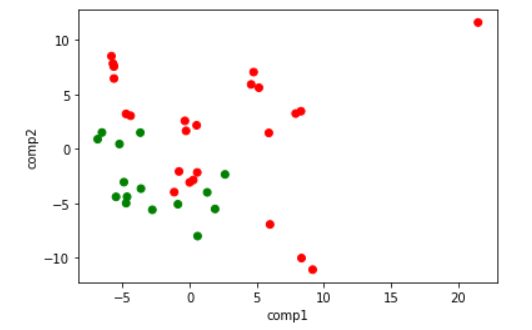
\includegraphics[width = 0.6\linewidth]{Capture 1.PNG}
    \caption{Plotting Principle Components 1 and 2}
    \label{fig:Capture 1}
\end{figure}
\begin{figure}[ht]
    \centering
    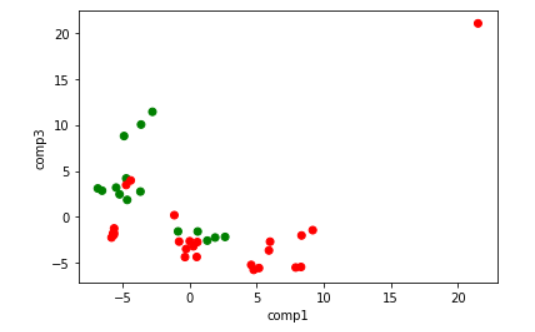
\includegraphics[width = 0.6\linewidth]{Capture 2.PNG}
    \caption{Plotting Principle Components 3 and 1}
    \label{fig:Capture 2}
\end{figure}
\begin{figure}[ht]
    \centering
    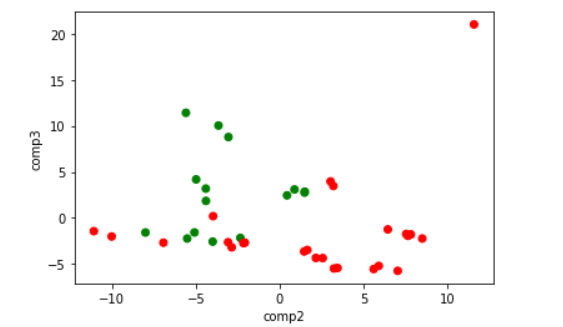
\includegraphics[width = 0.6\linewidth]{Capture 3.PNG}
    \caption{Plotting Principle Components 3 and 2}
    \label{fig:Capture 3}
\end{figure}


As we see from the charts above, the combination of Component 1 and Component 2 yields the best result. We also can see that outperforming data points are more associated with lower values for both Component 1 and Component 2, and thus can be tied to the negative words in those components, like "Energy", "Environment", "Competitive", "Demand", "Outbreak", etc.. 

All classifiers are then run using 5, 2 out of 3, and 2 principle components, looking at all metrics and assessing the performance of each of the classifiers. 

\clearpage
 
\begin{table}[!htb]
    \centering
    \begin{tabular}{c|c|c|c|c|c}
        \textbf{Data} & \textbf{Accuracy score} & \textbf{Recall Scores}& \textbf{Precision Scores}& \textbf{F1 Scores} \\
        \hline
        PC 1 and 2 out of 3 & 0.58 & 1., 0.25 & 0.73, 1. & 0.84, 0.4\\
        2 PC & 0.58 & 0.63, 0.5 & 0.71, 0.4 & 0.67, 0.44\\
        5 PC & 0.42 & 0.6, 0.29 & 0.38, 0.5 & 0.46, 0.36
    \end{tabular}
    \caption{Naive Bayes}
    \label{tab:Naive Bayes}
\end{table}


\begin{table}[!htb]
    \centering
    \begin{tabular}{c|c|c|c|c|c}
        \textbf{Data} & \textbf{Accuracy score} & \textbf{Recall Scores}& \textbf{Precision Scores}& \textbf{F1 Scores} \\
        \hline
        PC 1 and 2 out of 3 & 0.5 & 0.5, 0.5 & 0.67, 0.33 & 0.57, 0.4\\
        2 PC & 0.67 & 0.5, 1. & 1, 0.5 & 0.67, 0.67\\
        5 PC & 0.42 & 0.8, 0.14 & 0.4, 0.5 & 0.53, 0.22
    \end{tabular}
    \caption{KNN}
    \label{tab:KNN}
\end{table}

\begin{table}[!htb]
    \centering
    \begin{tabular}{c|c|c|c|c|c}
        \textbf{Data} & \textbf{Accuracy score} & \textbf{Recall Scores}& \textbf{Precision Scores}& \textbf{F1 Scores} \\
        \hline
        PC 1 and 2 out of 3 & 0.5 & 0.63, 0.25 & 0.63, 0.25 & 0.63, 0.25\\
        2 PC & 0.17 & 1, 0 & 0.83, 0 & 0.91, 0.\\
        5 PC & 0.5 & 0.6, 0.43 & 0.43, 0.6 & 0.5, 0.5
    \end{tabular}
    \caption{Logistic Regression}
    \label{tab:Logistic Regression}
\end{table}

\begin{table}[!htb]
    \centering
    \begin{tabular}{c|c|c|c|c|c}
        \textbf{Data} & \textbf{Accuracy score} & \textbf{Recall Scores}& \textbf{Precision Scores}& \textbf{F1 Scores} \\
        \hline
        PC 1 and 2 out of 3 & 0.5 & 0.5, 0.5 & 0.67, 0.33 & 0.57, 0.4\\
        2 PC & 0.58 & 1., 0. & 0.58, 0. & 0.74, 0.\\
        5 PC & 0.33 & 0.6, 0.14 & 0.33, 0.33 & 0.43, 0.2
    \end{tabular}
    \caption{Linear SVM}
    \label{tab:Linear SVM}
\end{table}


The results in tables \ref{tab:Naive Bayes}, \ref{tab:KNN}, \ref{tab:Logistic Regression}, and \ref{tab:Linear SVM} show that most of data/classifier combinations produce relatively low accuracy scores around or below 0.5. The highest accuracy score of 0.67 was achieved with a KNN classifier based on two principle components. The F1 Scores are relatively high for this classifier, however Recall and Precision Scores are not entirely conclusive. Overall, the better performance of KNN can be explained by the fact that this classifier works the best for non-linear data relationships (like stock market data). The selection of two principle components for this model is not arbitrary because, as it is stated in the dimensionality reduction section of the report, there is no clear cut off for selecting the number of principle component and theoretically, including more principle components would allow us more of the original variance in the data to be incorporated. 

Overall, for classification models the results of the experiments are inconclusive and need to be investigated further. Yet, several adjustments are recommended to be made:
\begin{itemize}
    \item Our data set is relatively small; we have around 20 instances of each class. Although such algorithms as Naive Bayes and KNN can work well with smaller data sets, the current results are inconclusive and need to be verified on a larger data set. We can expand it by adding results for more years, including annual reports of more companies or both.
    \item Neural Network classification can be used for classifying initial "bag of words" data sets into "classes", helping to mitigate bias introduced by filtering/reducing the subset of words manually.  
\end{itemize}



\clearpage
\section{Evaluation and final results}
The interpretation of the classification model results is critical to answer our research question. Unfortunately, the performance (in terms of accuracy) of all the models is not as strong as we would like. The remainder of this section focuses on the models with five principal components, as these also provide information on more strategies (e.g. mergers and acquisitions) compared to the two or three component models.

Our feature vector consists of five dimensions, which makes it impossible to plot directly in a 2 dimensional report. Figures \ref{fig:NB} and further help with this interpretation. Each plot contains of a grid of decision boundaries for two principal components at a time. The remaining three variables are kept constant at their mean value (which is zero because of the PCA procedure). 

Each grid is five by five, reflecting the five principal components that we considered in this step. The diagonal is empty; these would show decision boundaries where the x and y axis represent the same component, which is not in line with how decision boundaries are generally interpreted. The off-diagonal entries show the decision boundaries where the component on the x axis is given by the row number and the component on the y axis is given by the column number (which is labeled above the column). The following examples are based on the Naive Bayes classifications in Figure \ref{fig:NB}. For example, the bottom-left graph contains component 5 on the x-axis and component 1 on the y-axis. The top-right graph is exactly the same except for a switch in axes (i.e. component 1 is represented by the x axis and component 5 the y axis).

Going back to the bottom left graph, we can see that low values for component 1 (y axis) lead to underperformance (red). High values for this component indicate outperformance. We can judge the overall impact of a component by looking at the y axis under its label. For example, for component 1 we see that the top of the graph always tends to be "more green" than the bottom, hence high values for component 1 are indicative of outperformance. Some columns do not give a clear picture, such as those for component 2 and 4. 

It is important to remember that these visualizations are two dimensional slices through the origin of a five dimensional space. There may be other parts in the five dimensional space where the classification behaves differently. For example, the graph for the Naive Bayesian model clearly depicts the ellipsoid shape of the decision boundary in the first graph under component 4. 

In the next step, we decide for each component and model whether higher or lower values for the component lead to outperformance. Some of these remain undecided because of conflicting (or no) decision boundaries. For example, the KNN classification leads to very noisy predictions. Table \ref{tab:classification_results} contains the overall outcome based on all the graphs.

\begin{table}[ht]
    \centering
    \begin{tabular}{c|c|c|c|c|c}
        \textbf{Model} & \textbf{Component 1} & \textbf{Component 2}& \textbf{Component 3}& \textbf{Component 4}& \textbf{Component 5} \\
        \hline
        Naive Bayes & Higher & Undecided & Higher & Undecided & Undecided \\
        KNN & Undecided & Lower & Undecided & Undecided & Undecided \\
        Logistic Regression & Higher & Lower & Higher & Lower & Higher \\
        Linear SVM & Higher & Higher & Higher & Lower & Higher \\
        \hline
        Overall & Higher & Undecided & Higher & Lower & Higher 
    \end{tabular}
    \caption{Classification model results}
    \label{tab:classification_results}
\end{table}

The most likely strategy for outperformance has high values for components 1, 3 and 5, and low values for component 4. Reverting back to table \ref{tab:PCA_meaning} shows that this corresponds with a strategy that focuses on compliance issues, commercial aspects, the competitive environment, and mergers and acquisitions. The strategy should avoid focusing on catastrophes, financial aspects, and consumer needs. 

As the accuracy of the classification models were not particularly high, we can only treat this as a preliminary conclusion. There are several ways in which the analysis can be improved, namely:
\begin{itemize}
    \item The number of companies and years included in the data set can be increased to get more reliable results
    \item Models that take autocorrelation explicitly into account can be considered for more accurate modeling of text and returns over time
    \item The keyword selection in the bag of words model can be improved upon by starting with a defined set of words
    \item The bag of words model can be improved by also taking synonyms, similarity, and negation into account
    \item The dimensionality reduction step can be improved by trying other (non-linear) to capture more of the variability with less components
    \item The clustering section can be improved by considering different models or different distance metrics
    \item Classification models may be improved with further hyperparameter tuning (e.g. the number of neighbors in KNN)
    \item The translation from keywords to strategy should be done in cooperation with a (panel of) business strategy expert(s) to ensure that these are all viable strategies
\end{itemize}
Successful implementation of these steps may increase the accuracy of the classification models and our conviction of the (potentially new) conclusions.


\clearpage

\begin{figure}[htb]
    \centering
    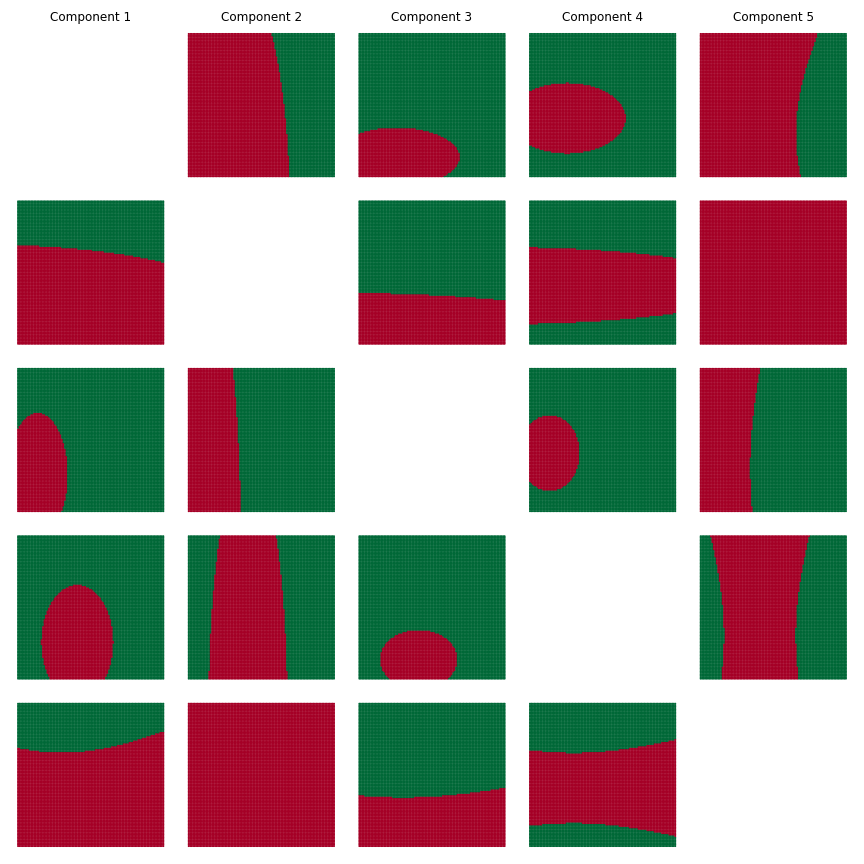
\includegraphics[width = 1.0\linewidth]{Naive Bayes_classification.png}
    \caption{Decision Boundaries Naive Bayes}
    \label{fig:NB}
\end{figure}
    
\begin{figure}[htb]
    \centering
    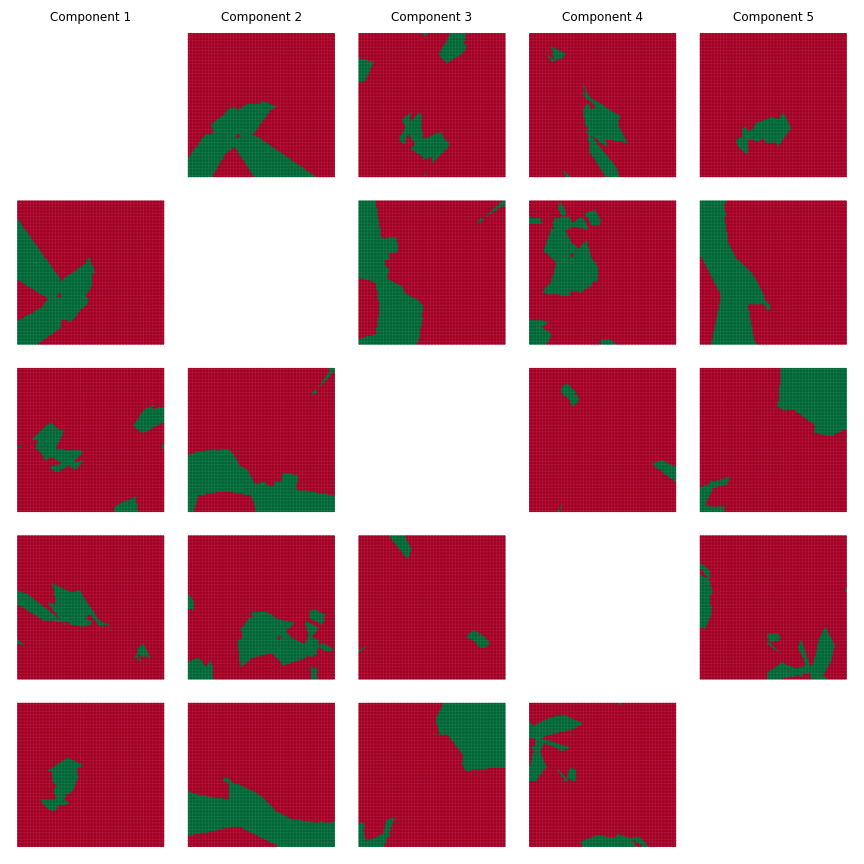
\includegraphics[width = 1.0\linewidth]{KNN_classification.png}
    \caption{Decision Boundaries KNN}
\end{figure}

\begin{figure}[htb]
    \centering
    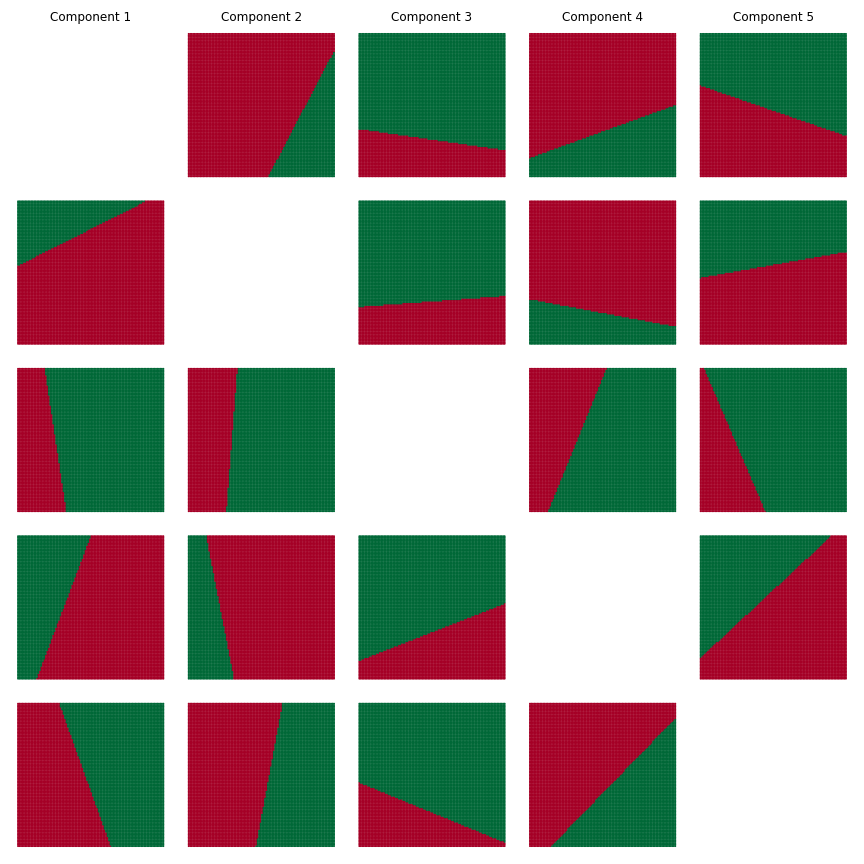
\includegraphics[width = 1.0\linewidth]{log_regression_classification.png}
    \caption{Decision Boundaries Logistic Regression}
\end{figure}

\begin{figure}[htb]
    \centering
    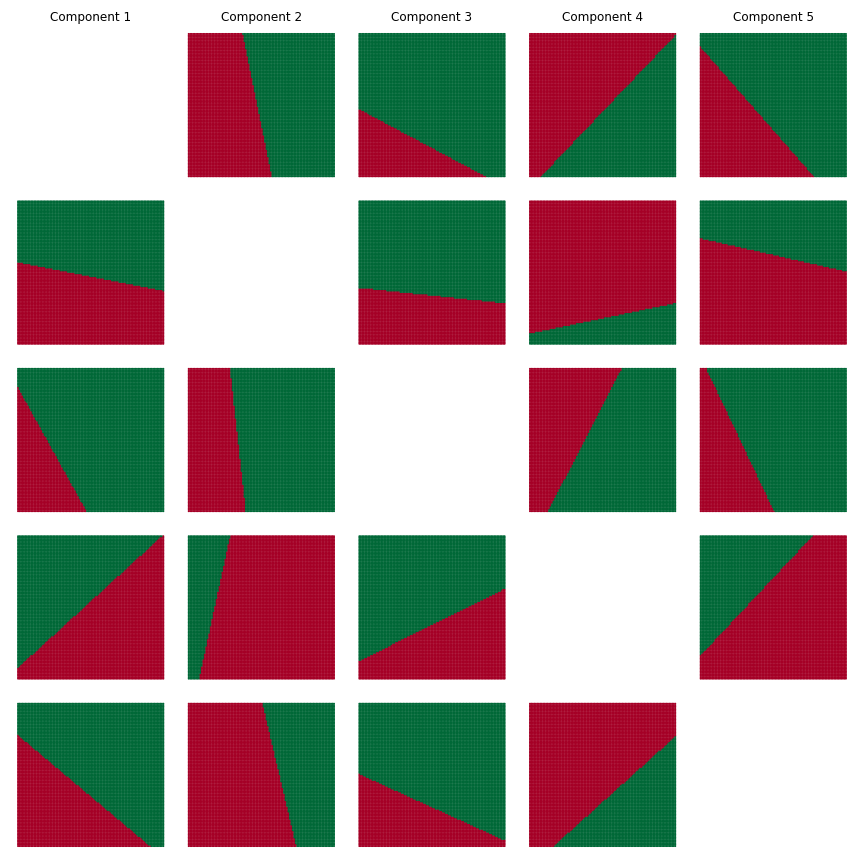
\includegraphics[width = 1.0\linewidth]{linear_svm_classification.png}
    \caption{Linear SVM Decision Boundaries}
\end{figure}

\clearpage
\section*{Appendix A: Who did what}
This section contains an overview of all the tasks the individual team members performed, in line with project requirements.

\vspace{5mm}
\textbf{Erik}
\begin{itemize}
    \item General
    \begin{itemize}
        \item Using \href{https://www.alphavantage.co/}{Alpha Vantage API} and \href{https://www.berkshirehathaway.com/letters/2019ltr.pdf}{Berkshire Hathaway reporting} to gather/transform financial data
        \item Code clean-up/reformatting for python notebook submissions
    \end{itemize}
    \item Report
    \begin{itemize}
        \item Section 2.2 Financial performance
        \item Section 3.1 Natural language processing (second half)
        \item Section 3.2 Dimensionality reduction (first half)
    \end{itemize}
    \item Coding
    \begin{itemize}
        \item exploratory\_data\_analysis.ipynb: exploring the annual report text data
        \item pca.ipynb: conducting principal component analysis
        \item stock\_data\_import.ipynb: collecting financial data from API
    \end{itemize}
\end{itemize}

\vspace{5mm}
\textbf{Jos}
\begin{itemize}
    \item General
    \begin{itemize}
        \item Initial idea, leading and taking minutes of project meetings 
        \item Keyword selection (bringing 5,651 unique words back to 422 business keywords)
        \item Wrote proposal
    \end{itemize}
    \item Report
    \begin{itemize}
        \item Section 1 Problem statement
        \item Section 2.1 Firm strategy
        \item Section 3.1 Natural language processing (first half)
        \item Section 3.2 Dimensionality reduction (second half)
        \item Section 3.3.1 Clustering
        \item Section 4 Evaluation and final results
    \end{itemize}
    \item Coding
    \begin{itemize}
        \item read\_txt.ipynb: reads text files and returns bag of words model
        \item clustering.ipynb: performs cluster analysis on five components
        \item Code to create the 5 by 5 decision bounds visualization
    \end{itemize}
\end{itemize}

\vspace{5mm}
\textbf{Vera}
\begin{itemize}
    \item General
    \begin{itemize}
        \item Searching and downloading annual reports from \href{https://www.annualreports.com/}{Annual Reports}
        \item Extracting data from annual reports and saving data in separate .txt files
    \end{itemize}
    \item Report
    \begin{itemize}
        \item Paragraph on data sourcing in Firm Strategy section 
        \item Full report on Classification in Classification and Clustering section
    \end{itemize}
    \item Coding
    \begin{itemize}
        \item File PCA + Models\_FINAL.ipynb (some PCA related code + Decision Boundaries code was prepared by Erik and Jos correspondingly, specific cells are commented in the Notebook) 
    \end{itemize}
\end{itemize}

\end{document}
